\chapter{Generative Models for Image Generation}
\label{chap:generative_models}

One of the most active and important areas of current machine learning research is the study of generative models. Unlike discriminative models, which
learn to map inputs to labels, generative models aim to learn the underlying
probability distribution of a dataset so that novel, realistic samples can be
synthesized. The capacity to model complex, high-dimensional distributions has
profound implications for image synthesis, data augmentation, representation
learning, and scientific simulation, among many other domains. The main families of deep generative models are comprehensively explored in this chapter, which examines their development from early probabilistic methods to current score-based and flow-based techniques.

% -------------------------------------------------------------------

\section{Overview of Deep Generative Models}
\label{sec:overview_generative}

A generative model is formally defined as a parametric approximation
$p_\theta(\mathbf{x})$ to an unknown data distribution $p_{\text{data}}(\mathbf{x})$,
where $\mathbf{x} \in \mathbb{R}^d$ and $\theta$ denotes the learnable parameters.
The central objective is to choose $\theta$ such that $p_\theta$ is, in some
well-defined sense, close to $p_{\text{data}}$. In practice, this closeness is
quantified by a divergence or distance measure — most commonly the
Kullback--Leibler (KL) divergence, the Jensen--Shannon divergence, or an
integral probability metric such as the Wasserstein distance
\cite{villani2009optimal}.

The history of statistical generative modeling predates the deep learning era,
encompassing classical approaches such as Gaussian mixture models, restricted
Boltzmann machines, and deep Boltzmann machines. However starting in the early 2010s, a significant change in the capabilities of generative models was brought about by the combination of large-scale datasets, advanced GPU hardware, and expressive neural network architecture.

Four major families can be used to classify modern deep generative models while also in Figure~\ref{fig:generative_taxonomy} there is an alternative categorization:
\begin{enumerate}
    \item \textbf{Variational Autoencoders (VAEs)} \cite{kingma2013auto,
    rezende2014stochastic}, which optimise a tractable lower bound on the
    log-likelihood through amortised variational inference;
    \item \textbf{Generative Adversarial Networks (GANs)} \cite{goodfellow2014generative},
    which frame generation as a two-player minimax game between a generator
    and a discriminator;
    \item \textbf{Diffusion and Score-Based Models}
    \cite{ho2020denoising, song2021scorebased}, which learn to reverse a
    stochastic noising process defined over a continuous time horizon; and
    \item \textbf{Normalising Flows and Flow Matching} \cite{chen2018neural,
    lipman2022flow}, which construct an invertible, differentiable mapping
    between a simple base distribution and the data manifold.
\end{enumerate}

\begin{figure}[ht]
    \centering
    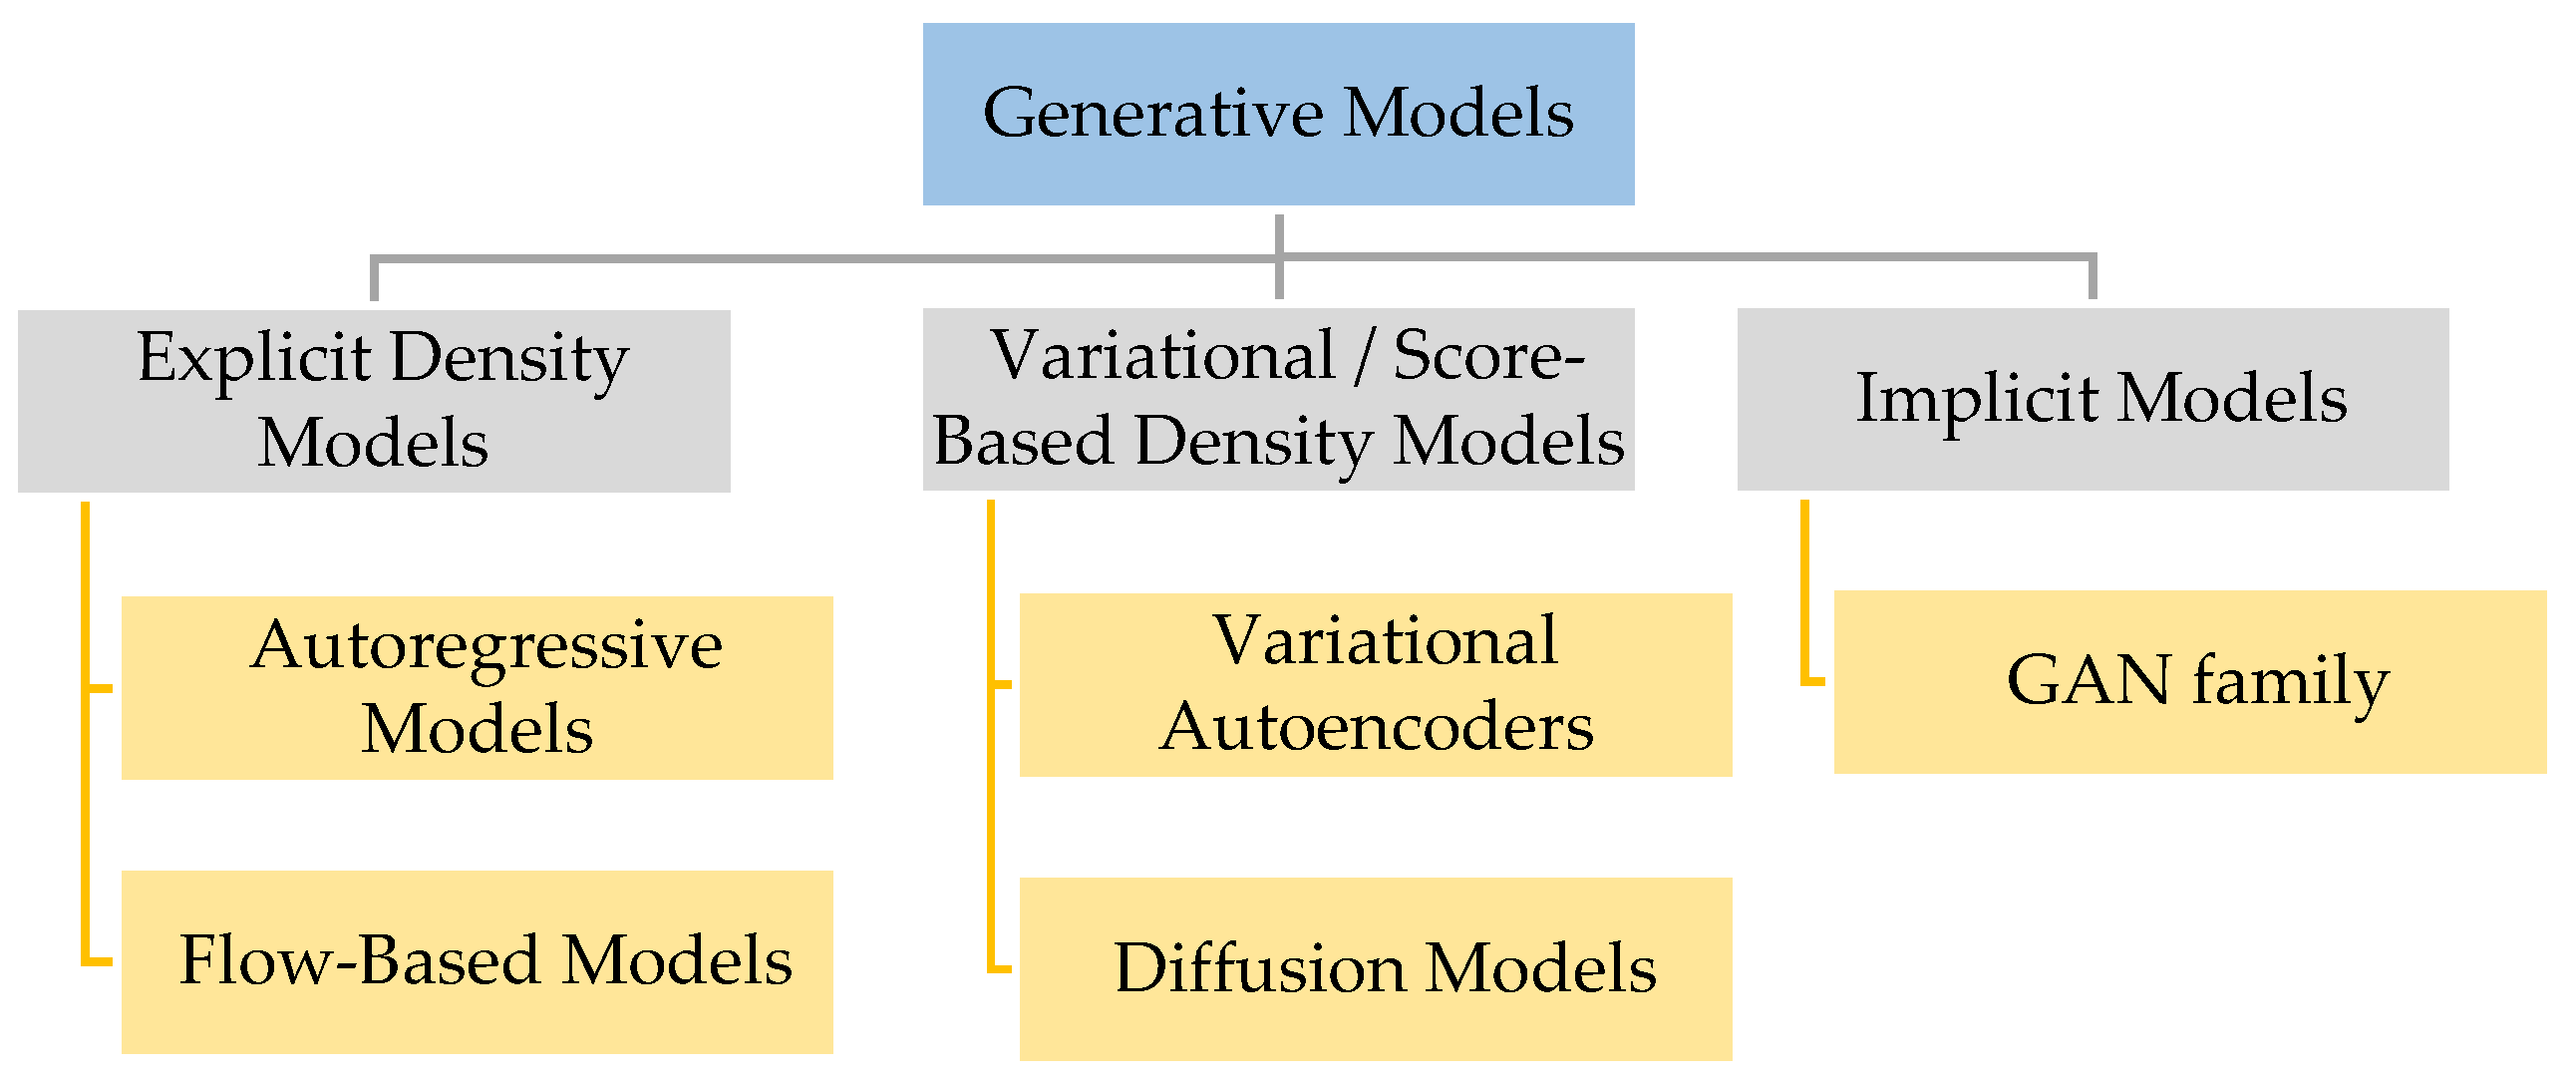
\includegraphics[width=0.92\linewidth]{figures/bcg/gen-models-taxonomy.png}
    \caption{A schematic taxonomy of the principal families of deep generative
    models. Each paradigm differs fundamentally in its training objective,
    inductive biases, and inference procedure.}
    \label{fig:generative_taxonomy}
\end{figure}

Each family embodies a distinct inductive bias and optimization strategy,
yielding characteristic trade-offs between sample quality, training stability,
mode coverage, and inference speed. The remainder of this chapter develops
the mathematical foundations of each paradigm in turn. This sets up the historical foundations before we move on and introduce our methodology in Chapter~\ref{chap:framework}

% -------------------------------------------------------------------

\section{Variational Autoencoders (VAEs)}
\label{sec:vaes}

Variational Autoencoders, introduced concurrently by Kingma and Welling
\cite{kingma2013auto} and Rezende, Mohamed, and Wierstra \cite{rezende2014stochastic},
provided one of the first scalable frameworks for approximate Bayesian inference
in deep latent variable models. The VAE posits a generative process in which
observations $\mathbf{x}$ are produced from latent variables
$\mathbf{z} \in \mathbb{R}^k$ via a learned decoder $p_\theta(\mathbf{x} \mid \mathbf{z})$,
combined with a prior $p(\mathbf{z})$ — typically an isotropic Gaussian
$\mathcal{N}(\mathbf{0}, \mathbf{I})$:

\begin{equation}
    p_\theta(\bm{x}) = \int p_\theta(\bm{x} \mid \bm{z})\, p(\bm{z})\, \mathrm{d}\bm{z}.
    \label{eq:vae_marginal}
\end{equation}

Because the integral in Equation~\ref{eq:vae_marginal} is intractable for
expressive decoders, direct maximum likelihood estimation is infeasible. The
VAE resolves this by introducing an approximate posterior (encoder)
$q_\phi(\mathbf{z} \mid \mathbf{x})$, parameterised by $\phi$, and optimising
the Evidence Lower Bound (ELBO):

\begin{equation}
    \mathcal{L}_{\text{ELBO}}(\theta, \phi;\, \mathbf{x}) =
    \mathbb{E}_{q_\phi(\mathbf{z} \mid \mathbf{x})}
    \bigl[\log p_\theta(\mathbf{x} \mid \mathbf{z})\bigr]
    - D_{\text{KL}}\bigl(q_\phi(\mathbf{z} \mid \mathbf{x}) \,\|\, p(\mathbf{z})\bigr),
    \label{eq:elbo}
\end{equation}

\noindent where $D_{\text{KL}}(\cdot \| \cdot)$ denotes the KL divergence. The
first term in Equation~\ref{eq:elbo} is a reconstruction likelihood that
encourages the decoder to faithfully recover the input, while the second term
acts as a regulariser that prevents the approximate posterior from deviating
arbitrarily from the prior. By jointly optimising $\theta$ and $\phi$ through
the \emph{reparameterisation trick} — which rewrites the expectation as
$\mathbf{z} = \boldsymbol{\mu}_\phi(\mathbf{x}) +
\boldsymbol{\sigma}_\phi(\mathbf{x}) \odot \boldsymbol{\epsilon}$,
$\boldsymbol{\epsilon} \sim \mathcal{N}(\mathbf{0}, \mathbf{I})$ — the ELBO
becomes differentiable with respect to both parameter sets, enabling
end-to-end training via stochastic gradient descent.

The VAE framework offered several decisive advantages over its predecessors.
First, it scales naturally to high-dimensional data through the use of deep
convolutional architectures for both encoder and decoder. Second, the learned
latent space is continuous and structured, facilitating smooth interpolation
between data points — a property with direct utility in representation learning
and data augmentation. Third, the probabilistic
formulation provides a principled mechanism for handling uncertainty.

Nonetheless, VAEs are subject to well-documented limitations. The KL term in
the ELBO encourages the posterior to collapse towards the prior when the
decoder is sufficiently expressive, a phenomenon termed \emph{posterior
collapse}. Furthermore, optimising the ELBO
under a simple Gaussian likelihood tends to produce blurry samples in
pixel space, as the model distributes probability mass broadly to minimise
the expected reconstruction error. Numerous
extensions have been proposed to mitigate these shortcomings, including
hierarchical VAEs and the introduction
of normalising flow posteriors \cite{rezende2015variational}. Nevertheless,
as image generation benchmarks evolved, adversarial and, ultimately, diffusion-based approaches gained more popularity,

% -------------------------------------------------------------------

\section{Generative Adversarial Networks (GANs)}
\label{sec:gans}

Generative Adversarial Networks, proposed by Goodfellow et al.\
\cite{goodfellow2014generative}, reconceived image synthesis as a competitive
game between two neural networks: a \emph{generator} $G_\theta : \mathcal{Z}
\to \mathcal{X}$ that maps samples from a simple latent distribution
$p_\mathbf{z}(\mathbf{z})$ to the data space, and a \emph{discriminator}
$D_\phi : \mathcal{X} \to [0, 1]$ that attempts to distinguish real samples
from generated ones. The original formulation casts this as the following
minimax problem:

\begin{equation}
    \min_\theta \max_\phi \; \mathcal{V}(G_\theta, D_\phi) =
    \mathbb{E}_{\mathbf{x} \sim p_{\text{data}}}[\log D_\phi(\mathbf{x})]
    + \mathbb{E}_{\mathbf{z} \sim p_\mathbf{z}}
    [\log(1 - D_\phi(G_\theta(\mathbf{z})))].
    \label{eq:gan_objective}
\end{equation}

At the theoretical optimum, the discriminator $D_\phi^*(\mathbf{x}) =
p_{\text{data}}(\mathbf{x}) / (p_{\text{data}}(\mathbf{x}) + p_\theta(\mathbf{x}))$
and the generator objective reduces to minimising the Jensen--Shannon divergence
between $p_{\text{data}}$ and $p_\theta$ \cite{goodfellow2014generative}.
Critically, the generator never accesses the training data directly; it
receives gradient information solely through the discriminator, thereby
circumventing the need for an explicit likelihood model. This implicit
generative approach unlocks a substantially richer hypothesis class for the
generator, yielding significantly sharper samples than the VAE under
comparable architectural budgets.

There was a rapid growth in the GAN framework in the years after its initial introduction. The Deep Convolutional GAN (DCGAN)
demonstrated that architectural guidelines — such as the use of strided
convolutions, batch normalisation, and the avoidance of pooling layers — were
essential for stable training. Subsequent theoretical analyses revealed that
the Jensen--Shannon divergence underlying Equation~\ref{eq:gan_objective}
is poorly behaved when the supports of $p_{\text{data}}$ and $p_\theta$ are
disjoint, a condition commonly encountered early in training. The Wasserstein
GAN (WGAN) addressed this by replacing the
JS divergence with the earth mover's distance:

\begin{equation}
    W(p_{\text{data}}, p_\theta) =
    \sup_{\|f\|_L \leq 1} \mathbb{E}_{\mathbf{x} \sim p_{\text{data}}}[f(\mathbf{x})]
    - \mathbb{E}_{\hat{\mathbf{x}} \sim p_\theta}[f(\hat{\mathbf{x}})],
    \label{eq:wasserstein}
\end{equation}

\noindent where the supremum is taken over all 1-Lipschitz functions $f$.
This reformulation yields more meaningful gradients throughout training and
substantially improves stability. The practical enforcement of the Lipschitz
constraint was subsequently refined through gradient penalty regularisation.

Progressive training strategies \cite{karras2018progressive} and large-scale
normalisation techniques further expanded the resolution ceiling of GAN
synthesis. The StyleGAN series demonstrated state-of-the-art perceptual quality on
high-resolution face generation by introducing a style-based generator
architecture that disentangles coarse and fine-grained attributes in the
latent space. Concurrently, large-scale class-conditional models such as
BigGAN pushed the Fréchet Inception Distance (FID)
\cite{heusel2017gans} on ImageNet to levels previously considered
unattainable, establishing GANs as the dominant paradigm for high-fidelity
image synthesis through the late 2010s.

\begin{figure}[ht]
    \centering
    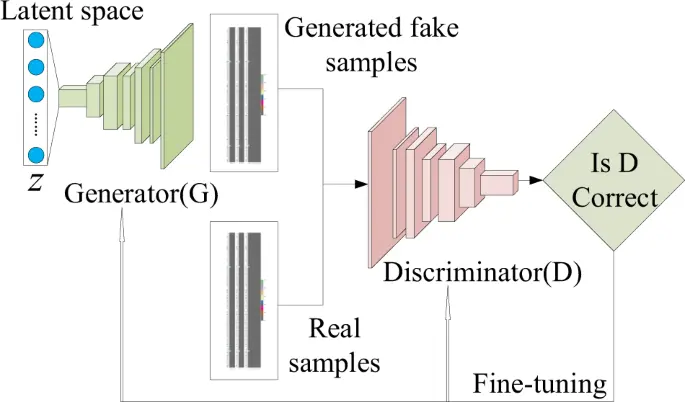
\includegraphics[width=0.85\linewidth]{figures/bcg/GAN.png}
    \caption{Schematic illustration of the GAN training procedure. The generator
    $G_\theta$ maps latent vectors $\mathbf{z}$ to synthetic images, while the
    discriminator $D_\phi$ produces a real/fake classification score.
    Gradients flow from $D_\phi$ back through $G_\theta$, with no direct access
    to the training data.}
    \label{fig:gan_diagram}
\end{figure}

Despite their impressive empirical performance, GANs are afflicted by several
fundamental difficulties. Training instability — characterised by oscillating
losses, gradient vanishing in the discriminator, and sensitivity to
hyperparameter choices — has been widely documented \cite{salimans2016improved}.
Mode collapse, wherein the generator produces samples of high perceptual
quality but low diversity, represents a particularly acute failure mode:
the generator may identify a small subset of the data manifold that reliably
deceives the discriminator and exploit it exclusively, thereby failing to
cover $p_{\text{data}}$ in its entirety . The
adversarial training objective provides no explicit mechanism for diversity
enforcement, and the practical mitigations — minibatch discrimination
\cite{salimans2016improved}, unrolled GANs — offer
only partial remedies. These intrinsic limitations, combined with the
comparatively greater training stability of likelihood-based methods, motivated
renewed interest in alternative generative paradigms, and ultimately contributed
to the ascendance of diffusion-based models as the dominant framework for
high-quality image synthesis \cite{dhariwal2021diffusion}.









































\section{Diffusion and Score-Based Generative Models}
\label{sec:diffusion}

Diffusion-based generative models represent a paradigm shift in the design of
deep generative systems, achieving unprecedented levels of sample fidelity and
diversity on complex image distributions \cite{dhariwal2021diffusion}. In
contrast to GANs, which rely on an adversarial training signal, or VAEs, which
optimise a variational lower bound on the likelihood, diffusion models learn to
reverse a stochastic \emph{noising process} that gradually destroys structure
in the data. The generative procedure is then conceived as the time-reversal
of this destruction: beginning from pure noise, the model iteratively denoises
a latent state until a coherent sample is recovered. This section develops the
mathematical foundations of the three principal formulations of this idea:
Denoising Diffusion Probabilistic Models (DDPMs), score-based generative
modelling via score matching, and the unifying perspective achieved through
stochastic differential equations (SDEs).

% -------------------------------------------------------------------

\subsection{Denoising Diffusion Probabilistic Models}
\label{subsec:ddpm}

Denoising Diffusion Probabilistic Models, introduced by Ho et al.\
\cite{ho2020denoising} and building upon the foundational work of Sohl-Dickstein
et al.\ \cite{sohl2015deep}, define a latent variable model over a sequence of
variables $\mathbf{x}_0, \mathbf{x}_1, \ldots, \mathbf{x}_T$, where
$\mathbf{x}_0 \sim p_{\text{data}}$ denotes a clean data sample and
$\mathbf{x}_T$ is approximately distributed as an isotropic Gaussian
$\mathcal{N}(\mathbf{0}, \mathbf{I})$ for a sufficiently large $T$.

\paragraph{The Forward Process.}
The \emph{forward} (or \emph{diffusion}) process $q$ is a fixed, non-learnable
Markov chain that incrementally corrupts the data by adding small amounts of
Gaussian noise at each step $t \in \{1, \ldots, T\}$:

\begin{equation}
    q(\mathbf{x}_t \mid \mathbf{x}_{t-1}) =
    \mathcal{N}\!\left(\mathbf{x}_t;\;
    \sqrt{1 - \beta_t}\,\mathbf{x}_{t-1},\; \beta_t \mathbf{I}\right),
    \label{eq:ddpm_forward_step}
\end{equation}

\noindent where $\{\beta_t\}_{t=1}^T \subset (0, 1)$ is a fixed variance
schedule, typically chosen to be monotonically increasing. A key analytical
benefit of this Markov structure is that the marginal $q(\mathbf{x}_t
\mid \mathbf{x}_0)$ is available in closed form. Defining
$\alpha_t = 1 - \beta_t$ and $\bar{\alpha}_t = \prod_{s=1}^{t} \alpha_s$,
one obtains:

\begin{equation}
    q(\mathbf{x}_t \mid \mathbf{x}_0) =
    \mathcal{N}\!\left(\mathbf{x}_t;\;
    \sqrt{\bar{\alpha}_t}\,\mathbf{x}_0,\;
    (1 - \bar{\alpha}_t)\mathbf{I}\right),
    \label{eq:ddpm_marginal}
\end{equation}

which allows arbitrary noisy latents to be sampled from $\mathbf{x}_0$
in a single step via the reparameterisation
$\mathbf{x}_t = \sqrt{\bar{\alpha}_t}\,\mathbf{x}_0 +
\sqrt{1 - \bar{\alpha}_t}\,\boldsymbol{\epsilon}$,
$\boldsymbol{\epsilon} \sim \mathcal{N}(\mathbf{0}, \mathbf{I})$.
This property is fundamental to the efficient training procedure described
below.

\paragraph{The Reverse Process.}
The \emph{reverse} (or \emph{generative}) process $p_\theta$ is a learned
Markov chain that operates in the opposite temporal direction, progressively
denoising a sample initialised from $\mathbf{x}_T \sim \mathcal{N}(\mathbf{0},
\mathbf{I})$:

\begin{equation}
    p_\theta(\mathbf{x}_{t-1} \mid \mathbf{x}_t) =
    \mathcal{N}\!\left(\mathbf{x}_{t-1};\;
    \boldsymbol{\mu}_\theta(\mathbf{x}_t, t),\;
    \Sigma_\theta(\mathbf{x}_t, t)\right).
    \label{eq:ddpm_reverse}
\end{equation}

The true reverse posterior $q(\mathbf{x}_{t-1} \mid \mathbf{x}_t, \mathbf{x}_0)$
is tractable and Gaussian when conditioned on $\mathbf{x}_0$:

\begin{equation}
    q(\mathbf{x}_{t-1} \mid \mathbf{x}_t, \mathbf{x}_0) =
    \mathcal{N}\!\left(\mathbf{x}_{t-1};\;
    \tilde{\boldsymbol{\mu}}_t(\mathbf{x}_t, \mathbf{x}_0),\;
    \tilde{\beta}_t \mathbf{I}\right),
    \label{eq:ddpm_posterior}
\end{equation}

\noindent with $\tilde{\boldsymbol{\mu}}_t(\mathbf{x}_t, \mathbf{x}_0) =
\frac{\sqrt{\bar{\alpha}_{t-1}}\beta_t}{1 - \bar{\alpha}_t}\mathbf{x}_0 +
\frac{\sqrt{\alpha_t}(1 - \bar{\alpha}_{t-1})}{1 - \bar{\alpha}_t}\mathbf{x}_t$
and $\tilde{\beta}_t = \frac{1 - \bar{\alpha}_{t-1}}{1 - \bar{\alpha}_t}\beta_t$.

\paragraph{Training Objective.}
Training proceeds by minimising a variational upper bound on the negative
log-likelihood, which decomposes over diffusion steps. Ho et al.\
\cite{ho2020denoising} showed that, after several simplifications, the
dominant contribution reduces to a reweighted denoising objective. In its
most widely adopted form, the model is parameterised as a noise-prediction
network $\boldsymbol{\epsilon}_\theta(\mathbf{x}_t, t)$, and the training
loss is:

\begin{equation}
    \mathcal{L}_{\text{simple}}(\theta) =
    \mathbb{E}_{t,\, \mathbf{x}_0,\, \boldsymbol{\epsilon}}
    \left[\left\|
    \boldsymbol{\epsilon} -
    \boldsymbol{\epsilon}_\theta\!\left(
    \sqrt{\bar{\alpha}_t}\,\mathbf{x}_0 +
    \sqrt{1 - \bar{\alpha}_t}\,\boldsymbol{\epsilon},\; t
    \right)
    \right\|^2\right],
    \label{eq:ddpm_loss}
\end{equation}

\noindent where $t \sim \mathcal{U}\{1, \ldots, T\}$ and
$\boldsymbol{\epsilon} \sim \mathcal{N}(\mathbf{0}, \mathbf{I})$.
This objective is equivalent to denoising score matching at each noise level
\cite{vincent2011connection}, a connection that will be made explicit in the
following subsection. The practical implementation employs a time-conditioned
U-Net architecture \cite{ronneberger2015unet} with sinusoidal timestep
embeddings, a design choice that has since become standard across the field.

Despite achieving sample quality competitive with, and often surpassing, state-of-the-art
GANs on benchmarks such as CIFAR-10 and LSUN \cite{ho2020denoising}, the DDPM
framework incurs a significant computational cost at inference time. Generating
a single sample requires $T$ sequential neural function evaluations — typically
$T = 1000$ — rendering DDPMs substantially slower than single-pass generators
such as GANs. This inference bottleneck is the primary motivation for the
distillation techniques examined in Chapter~\ref{chap:knowledge_distillation}.

% -------------------------------------------------------------------

\subsection{Score-Based Modeling and Score Matching}
\label{subsec:score_matching}

In parallel with the development of DDPMs, Song and Ermon
\cite{song2019generative, song2020improved} developed a distinct but intimately
related framework grounded in the concept of the \emph{score function}.
For a probability distribution $p(\mathbf{x})$, the score function is defined
as the gradient of the log-density with respect to the data:

\begin{equation}
    \mathbf{s}(\mathbf{x}) = \nabla_{\mathbf{x}} \log p(\mathbf{x}).
    \label{eq:score_function}
\end{equation}

The score function encodes the direction of steepest ascent in log-probability
space and is defined without reference to the normalising constant $Z$ in
$p(\mathbf{x}) = \tilde{p}(\mathbf{x}) / Z$. This property is particularly
attractive, as normalising constants are generally intractable for deep energy-based
models. Given access to the score, samples can be generated via
\emph{Langevin dynamics}: starting from an arbitrary initial point
$\mathbf{x}_0$, the chain:

\begin{equation}
    \mathbf{x}_{i+1} = \mathbf{x}_i +
    \frac{\eta}{2}\nabla_{\mathbf{x}} \log p(\mathbf{x}_i) +
    \sqrt{\eta}\,\boldsymbol{\xi}_i, \quad
    \boldsymbol{\xi}_i \sim \mathcal{N}(\mathbf{0}, \mathbf{I}),
    \label{eq:langevin}
\end{equation}

converges in distribution to $p(\mathbf{x})$ as $\eta \to 0$ and the number
of steps tends to infinity. The generative modeling
task then reduces to learning a neural score estimator
$\mathbf{s}_\theta(\mathbf{x}) \approx \nabla_{\mathbf{x}} \log p(\mathbf{x})$.

\paragraph{Score Matching.}
Learning the score directly from data can be achieved through the
\emph{score matching} objective of Hyvärinen \cite{hyvarinen2005estimation}:

\begin{equation}
    \mathcal{J}_{\text{SM}}(\theta) =
    \mathbb{E}_{p(\mathbf{x})}\left[
    \frac{1}{2}\left\|\mathbf{s}_\theta(\mathbf{x})\right\|^2
    + \operatorname{tr}\!\left(\nabla_{\mathbf{x}} \mathbf{s}_\theta(\mathbf{x})\right)
    \right],
    \label{eq:score_matching}
\end{equation}

which avoids the intractable log-likelihood entirely. However, the trace of
the Jacobian in Equation~\ref{eq:score_matching} is computationally expensive
to evaluate for high-dimensional $\mathbf{x}$. \emph{Denoising score matching}
\cite{vincent2011connection} circumvents this by instead training the model
to predict the score of a noise-corrupted data distribution $q_\sigma(\tilde{\mathbf{x}}
\mid \mathbf{x}) = \mathcal{N}(\tilde{\mathbf{x}}; \mathbf{x}, \sigma^2 \mathbf{I})$:

\begin{equation}
    \mathcal{J}_{\text{DSM}}(\theta; \sigma) =
    \mathbb{E}_{\mathbf{x} \sim p_{\text{data}}}\,
    \mathbb{E}_{\tilde{\mathbf{x}} \sim q_\sigma(\cdot|\mathbf{x})}\left[
    \left\|\mathbf{s}_\theta(\tilde{\mathbf{x}}, \sigma) -
    \nabla_{\tilde{\mathbf{x}}} \log q_\sigma(\tilde{\mathbf{x}} \mid \mathbf{x})
    \right\|^2\right],
    \label{eq:denoising_score_matching}
\end{equation}

\noindent where $\nabla_{\tilde{\mathbf{x}}} \log q_\sigma(\tilde{\mathbf{x}} \mid \mathbf{x})
= -(\tilde{\mathbf{x}} - \mathbf{x}) / \sigma^2$. The minimiser of
$\mathcal{J}_{\text{DSM}}$ equals the score of the smoothed distribution,
and a direct algebraic substitution reveals that this is equivalent to
learning a noise predictor up to a constant scaling factor — precisely the
DDPM objective of Equation~\ref{eq:ddpm_loss}. This connection,
established rigorously by Ho et al.\ \cite{ho2020denoising}, demonstrates
that DDPMs and score-based models are, at the level of their training objectives,
equivalent formulations of the same underlying idea.

\paragraph{Noise Conditioning and Multi-Scale Estimation.}
A practical difficulty with score matching at a single noise level $\sigma$ is
that the score function becomes uninformative in low-density regions of
$p_{\text{data}}$, precisely where accurate estimation is most critical for
high-quality generation. Song and Ermon \cite{song2019generative, song2020improved}
addressed this by training a \emph{Noise Conditional Score Network} (NCSN) on a
geometric sequence of noise levels
$\{\sigma_i\}_{i=1}^L$ with $\sigma_1 > \sigma_2 > \cdots > \sigma_L \approx 0$,
and performing annealed Langevin dynamics during inference. At large $\sigma$,
the perturbed distribution covers the ambient space densely, enabling robust
initialisation; at small $\sigma$, the score estimate closely tracks the
original data distribution.

% -------------------------------------------------------------------

\subsection{A Unified Framework via SDEs}
\label{subsec:sde}

Song et al.\ \cite{song2021scorebased} provided a unifying perspective that
subsumes both DDPMs and NCSNs as special cases of a continuous-time framework
defined by stochastic differential equations (SDEs). In this formulation, the
discrete Markov chain of the DDPM is replaced by a continuous stochastic
process $\{\mathbf{x}(t)\}_{t \in [0, T]}$, where $t = 0$ corresponds to
clean data and $t = T$ to a tractable noise distribution. The forward
diffusion process is governed by an Itô SDE of the form:

\begin{equation}
    \mathrm{d}\mathbf{x} = \mathbf{f}(\mathbf{x}, t)\,\mathrm{d}t
    + g(t)\,\mathrm{d}\mathbf{w},
    \label{eq:forward_sde}
\end{equation}

\noindent where $\mathbf{f}(\cdot, t) : \mathbb{R}^d \to \mathbb{R}^d$ is
the \emph{drift} coefficient, $g : \mathbb{R} \to \mathbb{R}$ is the scalar
\emph{diffusion} coefficient, and $\mathbf{w}$ is a standard Wiener process
(Brownian motion). The transition kernel $p_{0t}(\mathbf{x}(t) \mid \mathbf{x}(0))$
is Gaussian for the affine drift functions used in practice, and the marginal
distributions $\{p_t\}_{t \in [0,T]}$ evolve from $p_0 = p_{\text{data}}$
towards a tractable prior $p_T \approx \mathcal{N}(\mathbf{0}, \sigma^2_{\max}\mathbf{I})$.

\paragraph{The Reverse-Time SDE.}
Anderson \cite{anderson1982reverse} showed that the time-reversal of a
diffusion process described by Equation~\ref{eq:forward_sde} is itself
an Itô SDE:

\begin{equation}
    \mathrm{d}\mathbf{x} = \left[
    \mathbf{f}(\mathbf{x}, t) -
    g(t)^2 \nabla_{\mathbf{x}} \log p_t(\mathbf{x})
    \right]\mathrm{d}t
    + g(t)\,\mathrm{d}\bar{\mathbf{w}},
    \label{eq:reverse_sde}
\end{equation}

\noindent where $\bar{\mathbf{w}}$ is a Wiener process running in reverse
time, and $\mathrm{d}t$ denotes an infinitesimal negative time increment.
The term $\nabla_{\mathbf{x}} \log p_t(\mathbf{x})$ is the \emph{time-dependent
score function} of the marginal distribution at time $t$. Crucially, if this
score function is known, the reverse SDE is fully specified and can be
integrated numerically to yield samples from $p_0$. The generative modelling
task therefore reduces to learning a time-indexed score network
$\mathbf{s}_\theta(\mathbf{x}, t) \approx \nabla_{\mathbf{x}} \log p_t(\mathbf{x})$,
trained via the continuous-time analogue of the denoising score matching
objective:

\begin{equation}
    \mathcal{L}_{\text{score}}(\theta) =
    \mathbb{E}_{t}\!\left\{
    \lambda(t)\,\mathbb{E}_{\mathbf{x}(0), \mathbf{x}(t)}\!\left[
    \left\|\mathbf{s}_\theta(\mathbf{x}(t), t) -
    \nabla_{\mathbf{x}(t)} \log p_{0t}(\mathbf{x}(t) \mid \mathbf{x}(0))
    \right\|^2\right]\right\},
    \label{eq:score_sde_loss}
\end{equation}

\noindent where $\lambda(t) > 0$ is a weighting function and the expectation
over $t$ is taken uniformly over $[0, T]$.

\paragraph{Special Cases and the Probability Flow ODE.}
The DDPM corresponds to the \emph{Variance Preserving} (VP) SDE, with drift
$\mathbf{f}(\mathbf{x}, t) = -\frac{1}{2}\beta(t)\mathbf{x}$ and diffusion
coefficient $g(t) = \sqrt{\beta(t)}$, where $\beta(t)$ is the continuous-time
analogue of the noise schedule. The NCSN framework of Song and Ermon corresponds
to the \emph{Variance Exploding} (VE) SDE, characterised by zero drift and
$g(t) = \sqrt{\mathrm{d}[\sigma^2(t)]/\mathrm{d}t}$. Both are unified within
the SDE framework of Equation~\ref{eq:forward_sde}--\ref{eq:reverse_sde}.

A particularly consequential consequence of the SDE perspective is the existence
of an associated \emph{probability flow ordinary differential equation} (ODE)
\cite{song2021scorebased}:

\begin{equation}
    \frac{\mathrm{d}\mathbf{x}}{\mathrm{d}t} =
    \mathbf{f}(\mathbf{x}, t) -
    \frac{1}{2}g(t)^2\,\nabla_{\mathbf{x}} \log p_t(\mathbf{x}),
    \label{eq:probability_flow_ode}
\end{equation}

which is a deterministic process sharing the same marginal distributions
$\{p_t\}$ as the reverse SDE. Integrating Equation~\ref{eq:probability_flow_ode}
with an off-the-shelf ODE solver, using $\mathbf{s}_\theta$ in place of the
true score, produces high-quality samples while enabling exact likelihood
computation via the \emph{instantaneous change of variables formula}
\cite{chen2018neural}. Moreover, the probability flow ODE provides the
theoretical basis for accelerated sampling: since the stochastic component
has been eliminated, higher-order deterministic solvers can traverse the
trajectory in far fewer function evaluations than stochastic samplers
\cite{song2021denoising, lu2022dpm}. This observation underpins a
broad family of inference-time acceleration methods, including DDIM
\cite{song2021denoising} and DPM-Solver \cite{lu2022dpm}, which
reduce the number of required neural function evaluations by one to two
orders of magnitude relative to naive ancestral sampling, and constitute
the immediate precursors to the knowledge distillation approaches examined
in Chapter~\ref{chap:knowledge_distillation}.

\begin{figure}[ht]
    \centering
    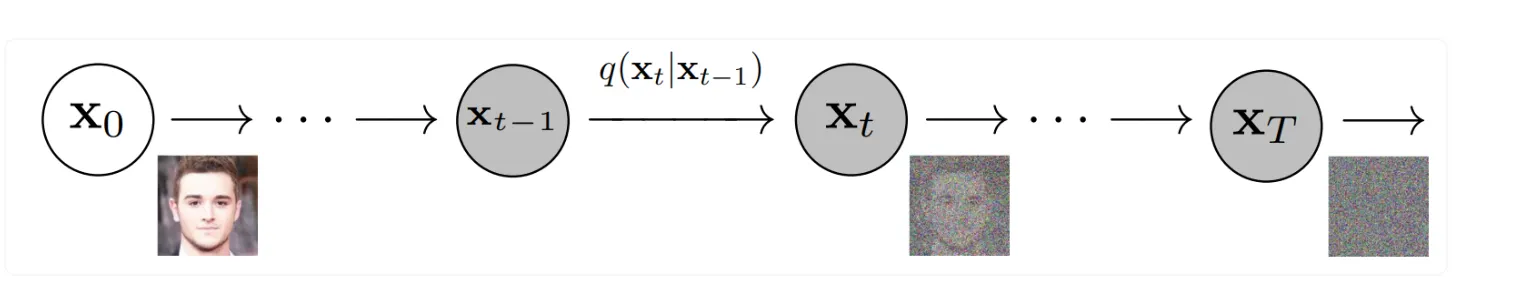
\includegraphics[width=0.95\linewidth]{figures/bcg/SFE-F-B.png}
    \caption{Illustration of the forward adiffusion processes in
    the SDE framework. The forward SDE (top) gradually corrupts data
    $\mathbf{x}(0) \sim p_{\text{data}}$ into noise $\mathbf{x}(T) \sim p_T$
    over continuous time}
    \label{fig:sde_forward_reverse}
\end{figure}

The SDE framework thus provides three practically significant contributions.
First, it provides a rigorous theoretical framework — grounded in stochastic
calculus — that bridges the relationship between previously distinct modeling concepts. Second, it decouples the \emph{design} of the forward process
(the choice of SDE) from the \emph{training} of the reverse model (score
matching), permitting principled exploration of novel noise schedules and
process geometries. Third, and most directly relevant to the present work,
the probability flow ODE reveals that the generative process of a diffusion
model can be expressed as a continuous trajectory in data space.


% =============================================================
\section{Flow Matching}
\label{sec:flow_matching}
% =============================================================

Diffusion models and score-based generative models, as discussed in the preceding sections,
construct a stochastic transport between a data distribution $p_{\text{data}}$ and a tractable
noise distribution through a \emph{fixed}, physically motivated degradation process. While
powerful, this design choice imposes constraints on training and inference efficiency:
the reverse process must be simulated over many discrete time steps, and the forward
noising schedule is not optimized for the geometry of the data. Flow matching constitutes
a complementary paradigm that frames generative modeling as the problem of learning a
\emph{deterministic} vector field whose associated ordinary differential equation (ODE)
transports samples from a source distribution to a target distribution in a principled,
simulation-free manner \cite{lipman2022flow, liu2022flow, albergo2023building}.
This section develops the theoretical foundations of flow matching, beginning with the
continuous normalizing flow framework, proceeding to the flow matching objective and
its conditional formulation, and concluding with the role of optimal transport and
rectified flows in producing straight, efficient trajectories.

% -------------------------------------------------------------
\subsection{Continuous Normalizing Flows}
\label{subsec:cnf}
% -------------------------------------------------------------

Normalizing flows define a family of generative models that express the data distribution
$p_1$ as an exact change-of-variables transformation of a simple base distribution
$p_0 = \mathcal{N}(\mathbf{0}, \mathbf{I})$. In discrete normalizing flows
\cite{rezende2015variational, dinh2016density}, this transformation is composed of a finite
sequence of invertible, differentiable mappings with analytically tractable Jacobian
determinants. Continuous normalizing flows (CNFs) \cite{chen2018neural} generalize this
construction by parameterizing the transformation as the solution to an autonomous
ordinary differential equation:

\begin{equation}
    \frac{d\mathbf{x}(t)}{dt} = v_\theta(\mathbf{x}(t),\, t), \quad t \in [0, 1],
    \label{eq:cnf_ode}
\end{equation}

\noindent where $\mathbf{x}(t) \in \mathbb{R}^d$ is the state of the system at time $t$,
and $v_\theta : \mathbb{R}^d \times [0,1] \to \mathbb{R}^d$ is a time-dependent vector
field parameterized by a neural network with parameters $\theta$. Given an initial
condition $\mathbf{x}(0) \sim p_0$, integrating the ODE in Equation~\ref{eq:cnf_ode}
forward in time from $t=0$ to $t=1$ yields a sample $\mathbf{x}(1) \sim p_1$, defining
the push-forward $p_1 = [\phi_1]_\# p_0$ where $\phi_t$ denotes the \emph{flow map}
associated with $v_\theta$.

The instantaneous change in log-density along a trajectory is governed by the
instantaneous change-of-variables formula \cite{chen2018neural}:

\begin{equation}
    \frac{d \log p_t(\mathbf{x}(t))}{dt} = -\nabla_{\mathbf{x}} \cdot v_\theta(\mathbf{x}(t), t),
    \label{eq:cnf_density}
\end{equation}

\noindent where $\nabla_{\mathbf{x}} \cdot v_\theta$ denotes the divergence of the
vector field. Equation~\ref{eq:cnf_density} enables exact likelihood computation by
integrating both the state and the log-density jointly; however, computing the
divergence in full generality requires $\mathcal{O}(d^2)$ operations or the use of
the Hutchinson stochastic trace estimator \cite{hutchinson1989stochastic}, which introduces
variance into training. Furthermore, CNF training requires solving an ODE at every
gradient step, rendering naive maximum-likelihood training computationally prohibitive
at scale. Flow matching addresses both of these limitations.

% -------------------------------------------------------------
\subsection{The Flow Matching Objective}
\label{subsec:flow_matching_objective}
% -------------------------------------------------------------

The central insight of flow matching \cite{lipman2022flow} is that one can train a CNF
without ever simulating the ODE during training, provided that a \emph{target} vector
field whose flow interpolates between $p_0$ and $p_1$ can be specified. Let
$p_t : [0,1] \to \mathcal{P}(\mathbb{R}^d)$ be a time-indexed probability path such
that $p_0 = \mathcal{N}(\mathbf{0}, \mathbf{I})$ and $p_1 \approx p_{\text{data}}$.
A vector field $u_t(\mathbf{x})$ is said to \emph{generate} the path $p_t$ if the
associated continuity equation is satisfied:

\begin{equation}
    \frac{\partial p_t(\mathbf{x})}{\partial t} + \nabla_{\mathbf{x}} \cdot \bigl(p_t(\mathbf{x})\, u_t(\mathbf{x})\bigr) = 0.
    \label{eq:continuity}
\end{equation}

The marginal flow matching (MFM) objective regresses the neural vector field $v_\theta$
directly onto $u_t$:

\begin{equation}
    \mathcal{L}_{\text{FM}}(\theta) = \mathbb{E}_{t \sim \mathcal{U}[0,1],\, \mathbf{x} \sim p_t}
    \bigl\| v_\theta(\mathbf{x}, t) - u_t(\mathbf{x}) \bigr\|^2.
    \label{eq:fm_loss}
\end{equation}

Although this objective is well-posed in principle, the marginal vector field $u_t(\mathbf{x})$
is generally intractable because it requires integrating over all data points that
could have generated a given noisy sample $\mathbf{x}$ at time $t$. Lipman et al.\
\cite{lipman2022flow} resolve this through the \emph{conditional flow matching} (CFM)
formulation. For each data sample $\mathbf{x}_1 \sim p_{\text{data}}$, one defines a
\emph{conditional} probability path $p_t(\mathbf{x} \mid \mathbf{x}_1)$ and an
associated conditional vector field $u_t(\mathbf{x} \mid \mathbf{x}_1)$, chosen such
that the marginals $p_t(\mathbf{x}) = \int p_t(\mathbf{x} \mid \mathbf{x}_1)\,
p_{\text{data}}(\mathbf{x}_1)\, d\mathbf{x}_1$ recover the desired path. The
conditional flow matching loss is then:

\begin{equation}
    \mathcal{L}_{\text{CFM}}(\theta) = \mathbb{E}_{t,\, \mathbf{x}_1 \sim p_{\text{data}},\,
    \mathbf{x} \sim p_t(\cdot \mid \mathbf{x}_1)}
    \bigl\| v_\theta(\mathbf{x}, t) - u_t(\mathbf{x} \mid \mathbf{x}_1) \bigr\|^2.
    \label{eq:cfm_loss}
\end{equation}

A key theoretical result establishes that $\mathcal{L}_{\text{CFM}}$ and
$\mathcal{L}_{\text{FM}}$ share identical gradients with respect to $\theta$
\cite{lipman2022flow}, meaning the conditional objective can be minimized in place of
the intractable marginal objective without any approximation. A natural and widely
adopted choice for the conditional path is the Gaussian interpolant:

\begin{align}
    p_t(\mathbf{x} \mid \mathbf{x}_1) &= \mathcal{N}\!\left(\mathbf{x};\; \mu_t(\mathbf{x}_1),\; \sigma_t^2 \mathbf{I}\right), \label{eq:gaussian_path}\\
    \mu_t(\mathbf{x}_1) &= \bigl(1 - (1 - \sigma_{\min})t\bigr)\,\mathbf{x}_0 + t\,\mathbf{x}_1, \label{eq:interpolant_mean}
\end{align}

\noindent with $\sigma_{\min} \ll 1$ controlling residual noise at $t=1$. The
corresponding conditional vector field admits the closed form:

\begin{equation}
    u_t(\mathbf{x} \mid \mathbf{x}_1) = \frac{\mathbf{x}_1 - (1 - \sigma_{\min})\mathbf{x}_0}
    {1 - (1 - \sigma_{\min})t},
    \label{eq:conditional_vf}
\end{equation}

\noindent which is a \emph{constant} vector field pointing from $\mathbf{x}_0$ to
$\mathbf{x}_1$ along a straight line. This observation has profound implications for
inference efficiency: if $v_\theta$ learns to reproduce straight-line trajectories, a
single Euler integration step suffices for generation, a property exploited directly
by consistency models \cite{song2023consistency} and rectified flows \cite{liu2022flow},
as discussed in Chapter~\ref{chap:knowledge_distillation}.

\begin{figure}[ht]
    \centering
    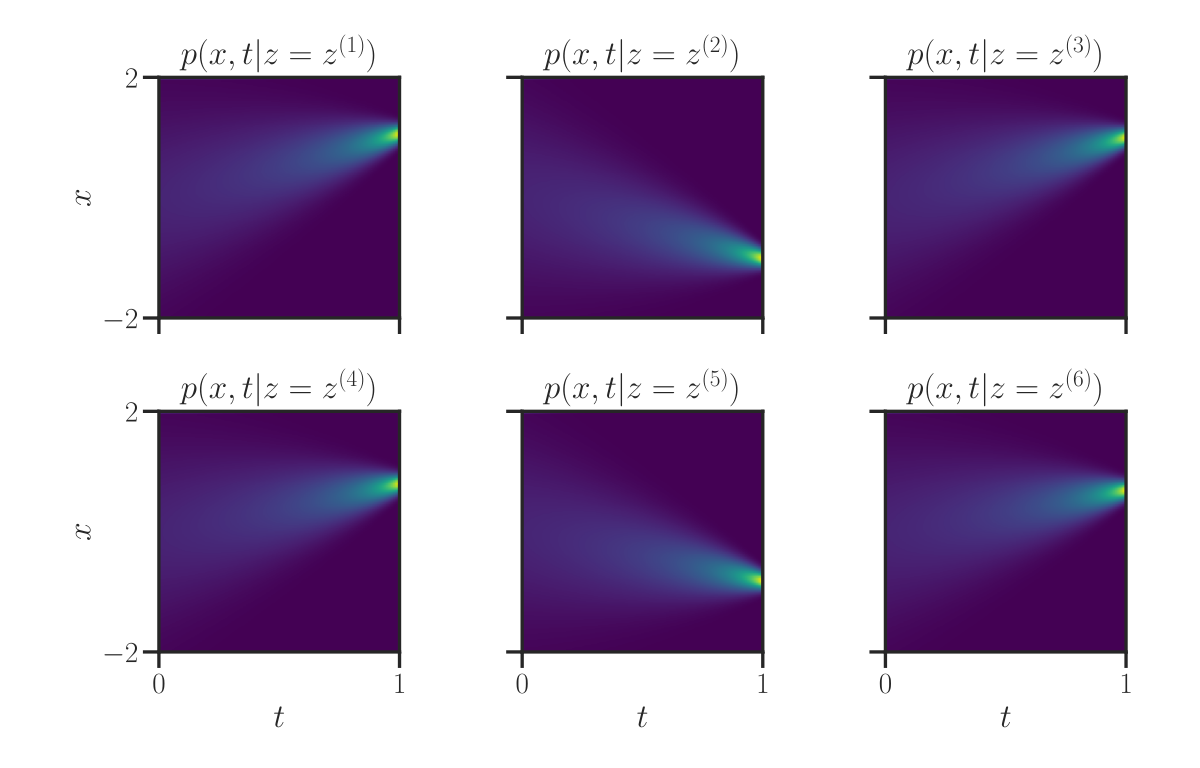
\includegraphics[width=0.85\linewidth]{figures/bcg/FM-CFM.png}
    \caption{Conditional probability paths as linear interpolation. $p(x|t, z = z^{(i)})$ for six samples $z^{(i)}$ (each being a pair $(x_0, x_1)$)}
    \label{fig:cfm_trajectories}
\end{figure}

% -------------------------------------------------------------
\subsection{Optimal Transport and Rectified Flows}
\label{subsec:ot_rectified}
% -------------------------------------------------------------

The freedom to specify the coupling between $p_0$ and $p_1$ in the CFM framework gives
rise to a natural optimization question: which coupling minimizes the average trajectory
length, and thus minimizes the integration error incurred during inference with a
finite-step ODE solver? This question is answered by the theory of optimal transport (OT)
\cite{villani2009optimal}.

Formally, given two distributions $p_0$ and $p_1$ on $\mathbb{R}^d$, the
$\ell^2$-optimal transport plan $\pi^* \in \mathcal{P}(\mathbb{R}^d \times \mathbb{R}^d)$
solves the Monge--Kantorovich problem:

\begin{equation}
    \pi^* = \underset{\pi \in \Pi(p_0,\, p_1)}{\arg\min}\;
    \mathbb{E}_{(\mathbf{x}_0, \mathbf{x}_1) \sim \pi}
    \bigl[\|\mathbf{x}_1 - \mathbf{x}_0\|^2\bigr],
    \label{eq:ot_problem}
\end{equation}

\noindent where $\Pi(p_0, p_1)$ denotes the set of all joint distributions with
marginals $p_0$ and $p_1$. $\pi^*$ is induced by a deterministic map $T^*$, i.e.\
$\pi^* = (\text{Id} \times T^*)_\# p_0$, and the optimal trajectories are straight
lines. Lipman et al.\ \cite{lipman2022flow} refer to the CFM variant that employs the
OT plan as \emph{OT-CFM}, and demonstrate empirically that it produces significantly
straighter flows and requires fewer function evaluations at inference time compared to
the independent coupling $\pi_{\text{ind}} = p_0 \otimes p_1$.

An independent but closely related approach, \emph{Rectified Flow} (RF) \cite{liu2022flow},
addresses the same problem of flow straightening through an iterative reflow procedure.
The core observation is that the linear interpolant between independently sampled pairs
$(\mathbf{x}_0, \mathbf{x}_1)$ defines a valid training target but may produce
trajectories that cross one another in data space, resulting in a non-straight marginal
vector field. Rectified flow proceeds as follows: given a coupling $\pi^{(k)}$ at
iteration $k$, one trains a vector field $v_\theta^{(k)}$ with the CFM loss under
$\pi^{(k)}$, generates paired samples $(\mathbf{x}_0, \hat{\mathbf{x}}_1)$ by
simulating $v_\theta^{(k)}$, and defines the refined coupling
$\pi^{(k+1)} = \text{Law}(\mathbf{x}_0, \hat{\mathbf{x}}_1)$. This reflow operation
progressively straightens trajectories, as proved in \cite{liu2022flow} through the
monotone decrease of the expected squared trajectory curvature.

The stochastic interpolants framework of Albergo and Vanden-Eijnden
\cite{albergo2023building} provides a unifying perspective that subsumes both flow
matching and score-based diffusion models. In that framework, an interpolant
$\mathbf{x}(t) = \alpha_t \mathbf{x}_1 + \beta_t \mathbf{x}_0 + \gamma_t \boldsymbol{\epsilon}$
with $\boldsymbol{\epsilon} \sim \mathcal{N}(\mathbf{0}, \mathbf{I})$ induces a
probability path whose generating vector field can be expressed either as a drift
(yielding an ODE) or as a drift-diffusion pair (yielding an SDE), depending on whether
$\gamma_t$ is identically zero. When $\gamma_t = 0$ and the coupling is the OT plan,
one recovers a deterministic OT-CFM; when $\gamma_t > 0$, the framework recovers
the DDPM forward process as a special case \cite{ho2020denoising}. This unification
demonstrates that diffusion models and flow-based models differ not in kind but in the
choice of trajectory geometry and stochasticity, a distinction with direct consequences
for the design of knowledge distillation strategies.

\begin{figure}[ht]
    \centering
    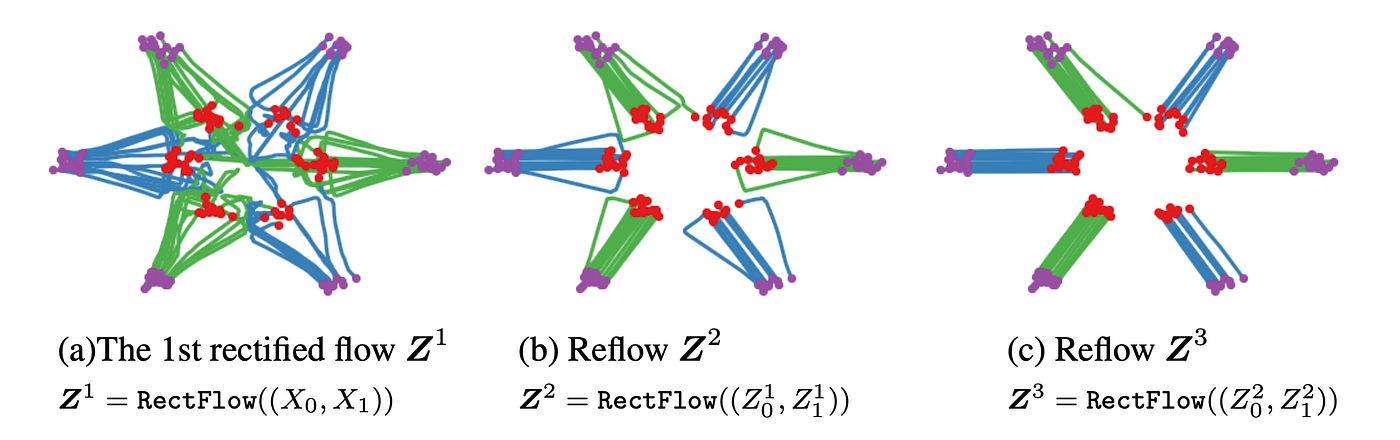
\includegraphics[width=0.82\linewidth]{figures/bcg/RF.png}
    \caption{Schematic of the rectified flow reflow procedure. a): an initial
    1-Rectified Flow trained on independent couplings exhibits crossing trajectories.
    b): after a single reflow step (2-Rectified Flow), trajectories become
    approximately straight. c): 3-Rectified Flow trajectories have become completely straight.}
    \label{fig:rectified_flow}
\end{figure}

In summary, flow matching provides a simulation-free, likelihood-free training framework
for continuous normalizing flows whose flexibility in specifying the probability path
and source-target coupling makes it highly desirable formulation in modern generative models architecture like the "Just Image Transformer" that we will see in Chapter~\ref{chap:architectures}.